En el presente capítulo se explica la experimentación 
realizada para la clasificación de los videos del 
\textit{dataset Hockey Fights}. La 
estructura que se detalla a continuación consiste de: 
explicación del \textit{pipeline}, la experimentación 
con las diferentes configuraciones de BI-LSTM y la 
comparativa de los resultados.

En la Sección \ref{software} se explican las especificaciones de 
\textit{software} y \textit{hardware} que se necesitaron para la 
realización del trabajo.\\

Mientras que en la Sección \ref{experimentacion} se detallan todos los experimentos 
realizados con cada una de las diferentes configuraciones y sus 
resultados.\\

Por último, en la Sección {comparativa} se realiza la comparativa de 
todos los resultados obtenidos considerando el promedio y las mejores 
ejecuciones del \textit{pipeline} para finalmente poder obtener una 
conclusión acerca de la influencia del número de capas Bi-LSTM con 
respecto a los resultados finales obtenidos. 

\section{Software y Hardware}\label{software}

A lo largo de toda la experimentación, se utiliza
un computador de escritorio. Los detalles de la misma se encuentran en 
la Tabla \ref{caracteristicas}.

\begin{table}[h!]
\centering
\caption{Características del computador utilizado para el trabajo.}

\begin{tabular}{|r|r|}
\hline
\textbf{Componente} & \textbf{Descripción} \\ \hline
Procesador & AMD Ryzen 7 3700X 8-Core 3.6 GHz. \\ \hline
Memoria RAM & Crucial Ballistix 16GB DDR4 - 3600MHZ \\ \hline
Tarjeta Gráfica & Nvidia RTX 2060 6GB \\ \hline
\end{tabular}
\label{caracteristicas}
\end{table}

Por otra parte, se utilizó Python, junto con Keras, Sklearn y Tensorflow 
para el desarrollo del \textit{pipeline} en general y el pre y post 
procesamiento de los datos. Para el procesamiento de las imágenes (con Yolo) 
se utilizó OpenCV compilado con cudnn para la habilitación del uso de tarjeta gráfica. 

\section{Experimentación} \label{experimentacion}

La presente Sección se subdivide en dos partes: la Sección \ref{procesamiento} 
revisa la creación de la CNN encargada de extraer las características de cada uno 
de los frames, mientras que la Sección \ref{clasificacion} presenta la 
experimentación de las diferentes configuraciones de la Bi-LSTM con múltiples 
capas.\\

En la Sección \ref{procesamiento} se detallan los pasos del 
procesamiento, los resultados provenientes del mismo y una tabla 
comparativa con métricas específicas por modelo de CNN a utilizar. 

Mientras que en la Sección \ref{clasificacion} se detallan los 
resultados obtenidos de utilizar diferentes configuraciones de capas 
Bi-LSTM para clasificar los vectores característicos obtenidos de los 
\textit{frames}. 


\subsection{Preprocesamiento y obtención de características}\label{procesamiento}

Como primer paso, se procede a realizar el pre-procesamiento 
de las imágenes y la obtención de sus características tal 
como fue mencionado anteriormente. Para ello, se utilizan los modelos 
con sus pesos preentrenados con el \textit{dataset ImageNet}. Además, se 
congelan todas sus capas convolucionales y eliminan todas las demás. Por último 
se agrega una capa \textit{GlobalAveragePooling2D}. Una vez terminado, 
se recolectan las métricas acerca de la cantidad de parámetros y el 
tiempo de cálculo por batch de cada uno de los modelos, los cuales 
se puden observar en la Tabla \ref{tabla:preprocesamiento}:

\begin{table}[h!]
\centering
\caption{Tabla comparativa de los parámetros y tiempo de inferencia por modelo.}
\begin{tabular}{|l|l|l|}
\hline
\multicolumn{1}{|c|}{\textbf{Modelo}} & \multicolumn{1}{c|}{\textbf{Parámetros}} & \multicolumn{1}{c|}{\textbf{\begin{tabular}[c]{@{}c@{}}Timpo de inferencia\\ (por batch de 10)\\ en ms/batch\end{tabular}}} \\ \hline
\textbf{Efficientnetb0}               & 4,049,571                                & 46 ms                                                                                                                       \\ \hline
\textbf{Resnet50}                     & 23,587,712                               & 51 ms                                                                                                                       \\ \hline
\textbf{Efficientnetv2-s}             & 20,331,360                               & 75 ms                                                                                                                       \\ \hline
\textbf{MobilenetV3large}             & 2,996,352                                & 45 ms                                                                                                                       \\ \hline
\end{tabular}
\label{tabla:preprocesamiento}
\end{table}

Se puede apreciar que el tamaño final de los modelos fue 
menor que el esperado por la Tabla \ref{evaluacion}. 
Esto se debe a que no se están utilizando las capas densas 
de los modelos y se estan reemplazando con una capa 
GlobalAveragePooling2D, la cual obtiene el resultado del 
kernel final de las capas convolucionales y las reduce a un 
solo resultado promediado. 

\subsection{Clasificación de los videos a través de la Bi-LSTM}\label{clasificacion}

Después de obtener las características de cada uno de las 
imágenes y los diez frames generados por cada uno de ellas, 
se entrenan diferentes modelos BI-LSTM como fue mencionado 
anteriormente, teniendo desde 1 a 10 celdas para cada uno de 
las CNN utilizados tal como se menciona en la Sección 
\ref{pipeline}. A continuación se explican los resultados para cada 
una de los diferentes experimentos realizados.\\

\textbf{\underline{Resultados obtenidos con EfficientNetB0}}\\

La Tabla \ref{table:b0Metrics} muestra una comparativa 
entre los resultados obtenidos para el \textit{pipeline} manteniendo 
los vectores de características obtenidas a través de EfficientNetB0 
de los frames del \textit{dataset Hockey Fights}.\\

\begin{table}[h!]
\centering
\footnotesize
\caption{Métricas obtenidas por configuración de celdas para EfficientNetB0.}
\begin{tabular}{|l|l|l|l|l|l|l|}
\hline
\textbf{\begin{tabular}[c]{@{}l@{}}Celdas \\ Bi-LSTM\end{tabular}} & \textbf{\begin{tabular}[c]{@{}l@{}}Perdida \\ entrenamiento\end{tabular}} & \textbf{\begin{tabular}[c]{@{}l@{}}Accuracy \\ entrenamiento\end{tabular}} & \textbf{\begin{tabular}[c]{@{}l@{}}Perdida \\ validacion\end{tabular}} & \textbf{\begin{tabular}[c]{@{}l@{}}Accuracy \\ validacion\end{tabular}} & \textbf{\begin{tabular}[c]{@{}l@{}}Perdida \\ prueba\end{tabular}} & \textbf{\begin{tabular}[c]{@{}l@{}}Accuracy \\ prueba\end{tabular}} \\ \hline
\textbf{1}                                                         & 0.07                                                                      & 0.98                                                                       & 0.22                                                                   & 0.94                                                                    & 0.12                                                               & 0.97                                                                \\ \hline
\textbf{2}                                                         & 0.05                                                                      & 0.99                                                                       & 0.1                                                                    & 0.98                                                                    & 0.08                                                               & 0.98                                                                \\ \hline
\textbf{3}                                                         & 0.04                                                                      & 0.99                                                                       & 0.16                                                                   & 0.96                                                                    & 0.08                                                               & 0.98                                                                \\ \hline
\textbf{4}                                                         & 0.02                                                                      & 0.99                                                                       & 0.14                                                                   & 0.95                                                                    & 0.08                                                               & 0.97                                                                \\ \hline
\textbf{5}                                                         & 0.02                                                                      & 0.99                                                                       & 0.16                                                                   & 0.96                                                                    & 0.07                                                               & 0.98                                                                \\ \hline
\textbf{6}                                                         & \textbf{0.0}                                                              & \textbf{1.0}                                                               & \textbf{0.15}                                                          & \textbf{0.98}                                                           & \textbf{0.03}                                                      & \textbf{0.99}                                                       \\ \hline
\textbf{7}                                                         & 0.05                                                                      & 0.99                                                                       & 0.19                                                                   & 0.96                                                                    & 0.13                                                               & 0.96                                                                \\ \hline
\textbf{8}                                                         & 0.03                                                                      & 0.99                                                                       & 0.14                                                                   & 0.98                                                                    & 0.06                                                               & 0.99                                                                \\ \hline
\textbf{9}                                                         & 0.02                                                                      & 0.99                                                                       & 0.14                                                                   & 0.98                                                                    & 0.09                                                               & 0.98                                                                \\ \hline
\end{tabular}
\label{table:b0Metrics}
\end{table}


En la Tabla \ref{table:b0Metrics} se puede observar 
que los mejores resultados a lo largo de todos los pasos del 
\textit{pipeline} fue la configuración de 6 celdas, generando 99\% de 
\textit{accuracy} en prueba. Además, se pudo observar que los 
resultados de las demás configuraciones fueron similares a lo largo de 
todas las confguraciones, pero si se revisa los valores entre ellas, 
es claro que todos ellos empeoran mientras más se alejan de esa 
configuración, salvo en la configuración con 6 celdas que es un caso 
anómalo.\\

A continuación se presentan las gráficas de pérdida y \textit{accuracy} 
de esta configuración.

\begin{figure}[h!] 
    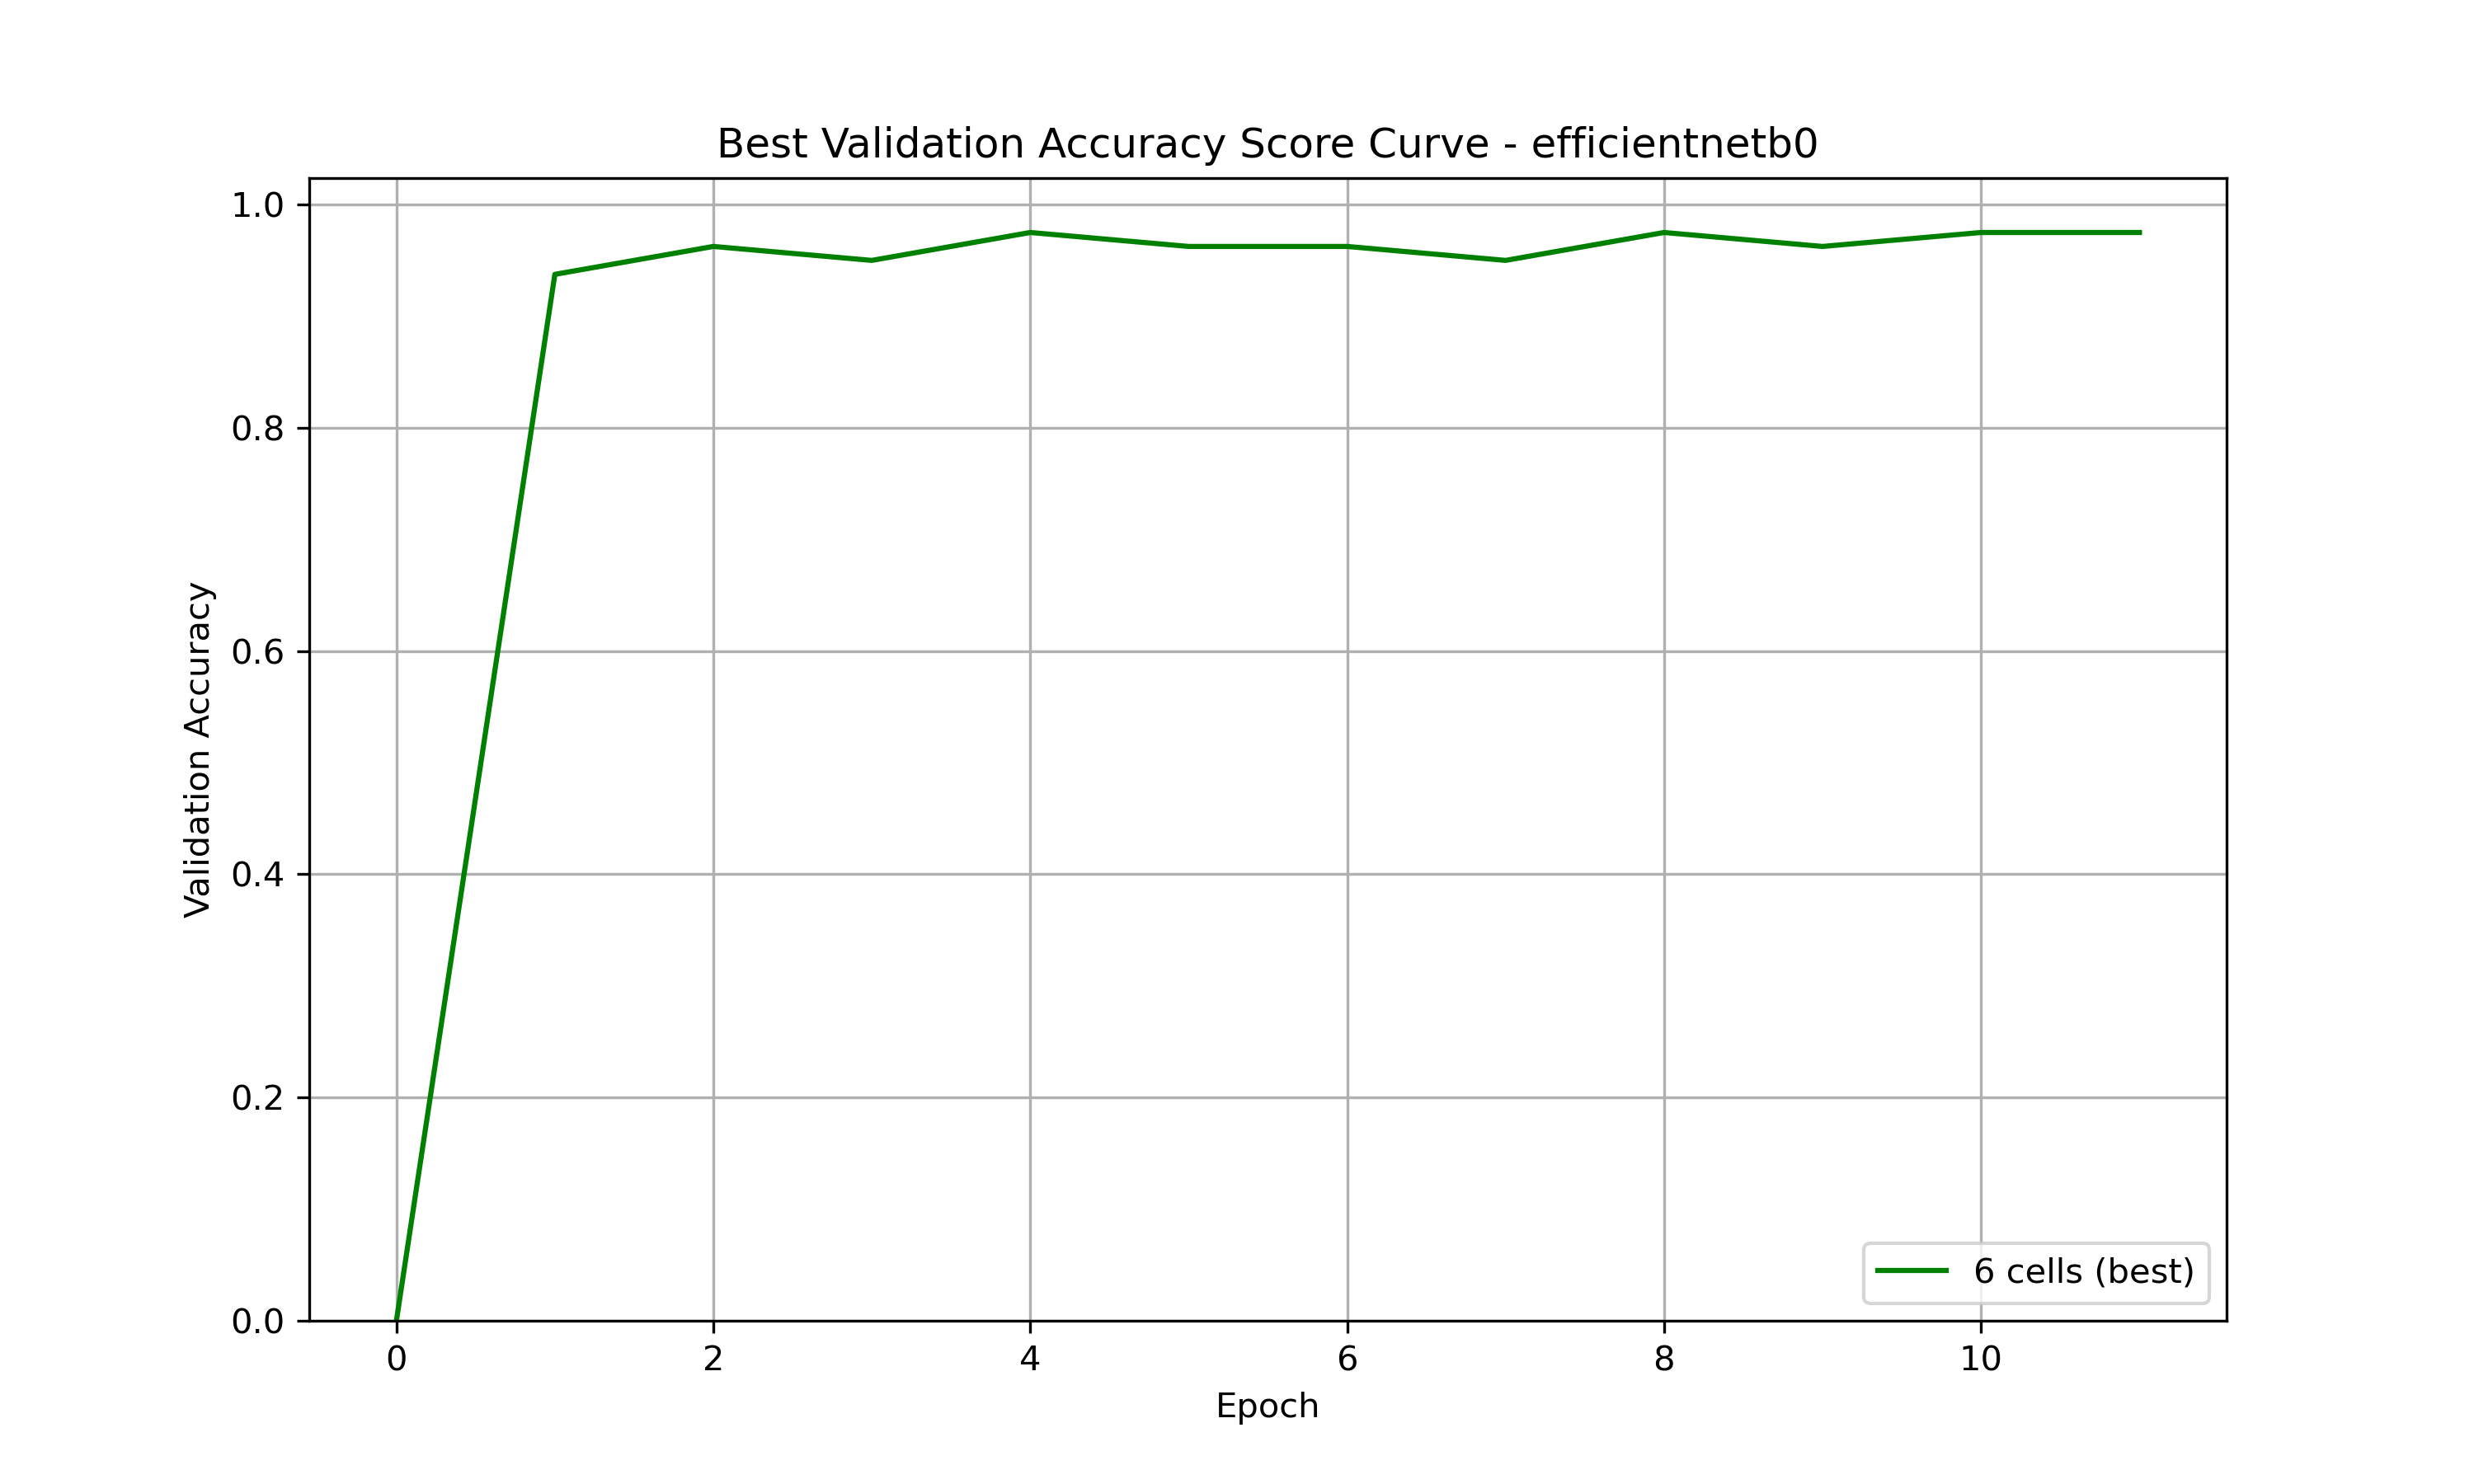
\includegraphics[width=0.8\textwidth]{../graphs/efficientnetb0_best_val_accuracy.png} 
    \centering 
    \caption{\textit{Accuracy} por época de EfficientNetB0 y 6 capas Bi-LSTM } 
    \label{EfficientNetB0Accuracy} 
\end{figure}

\begin{figure}[h!] 
    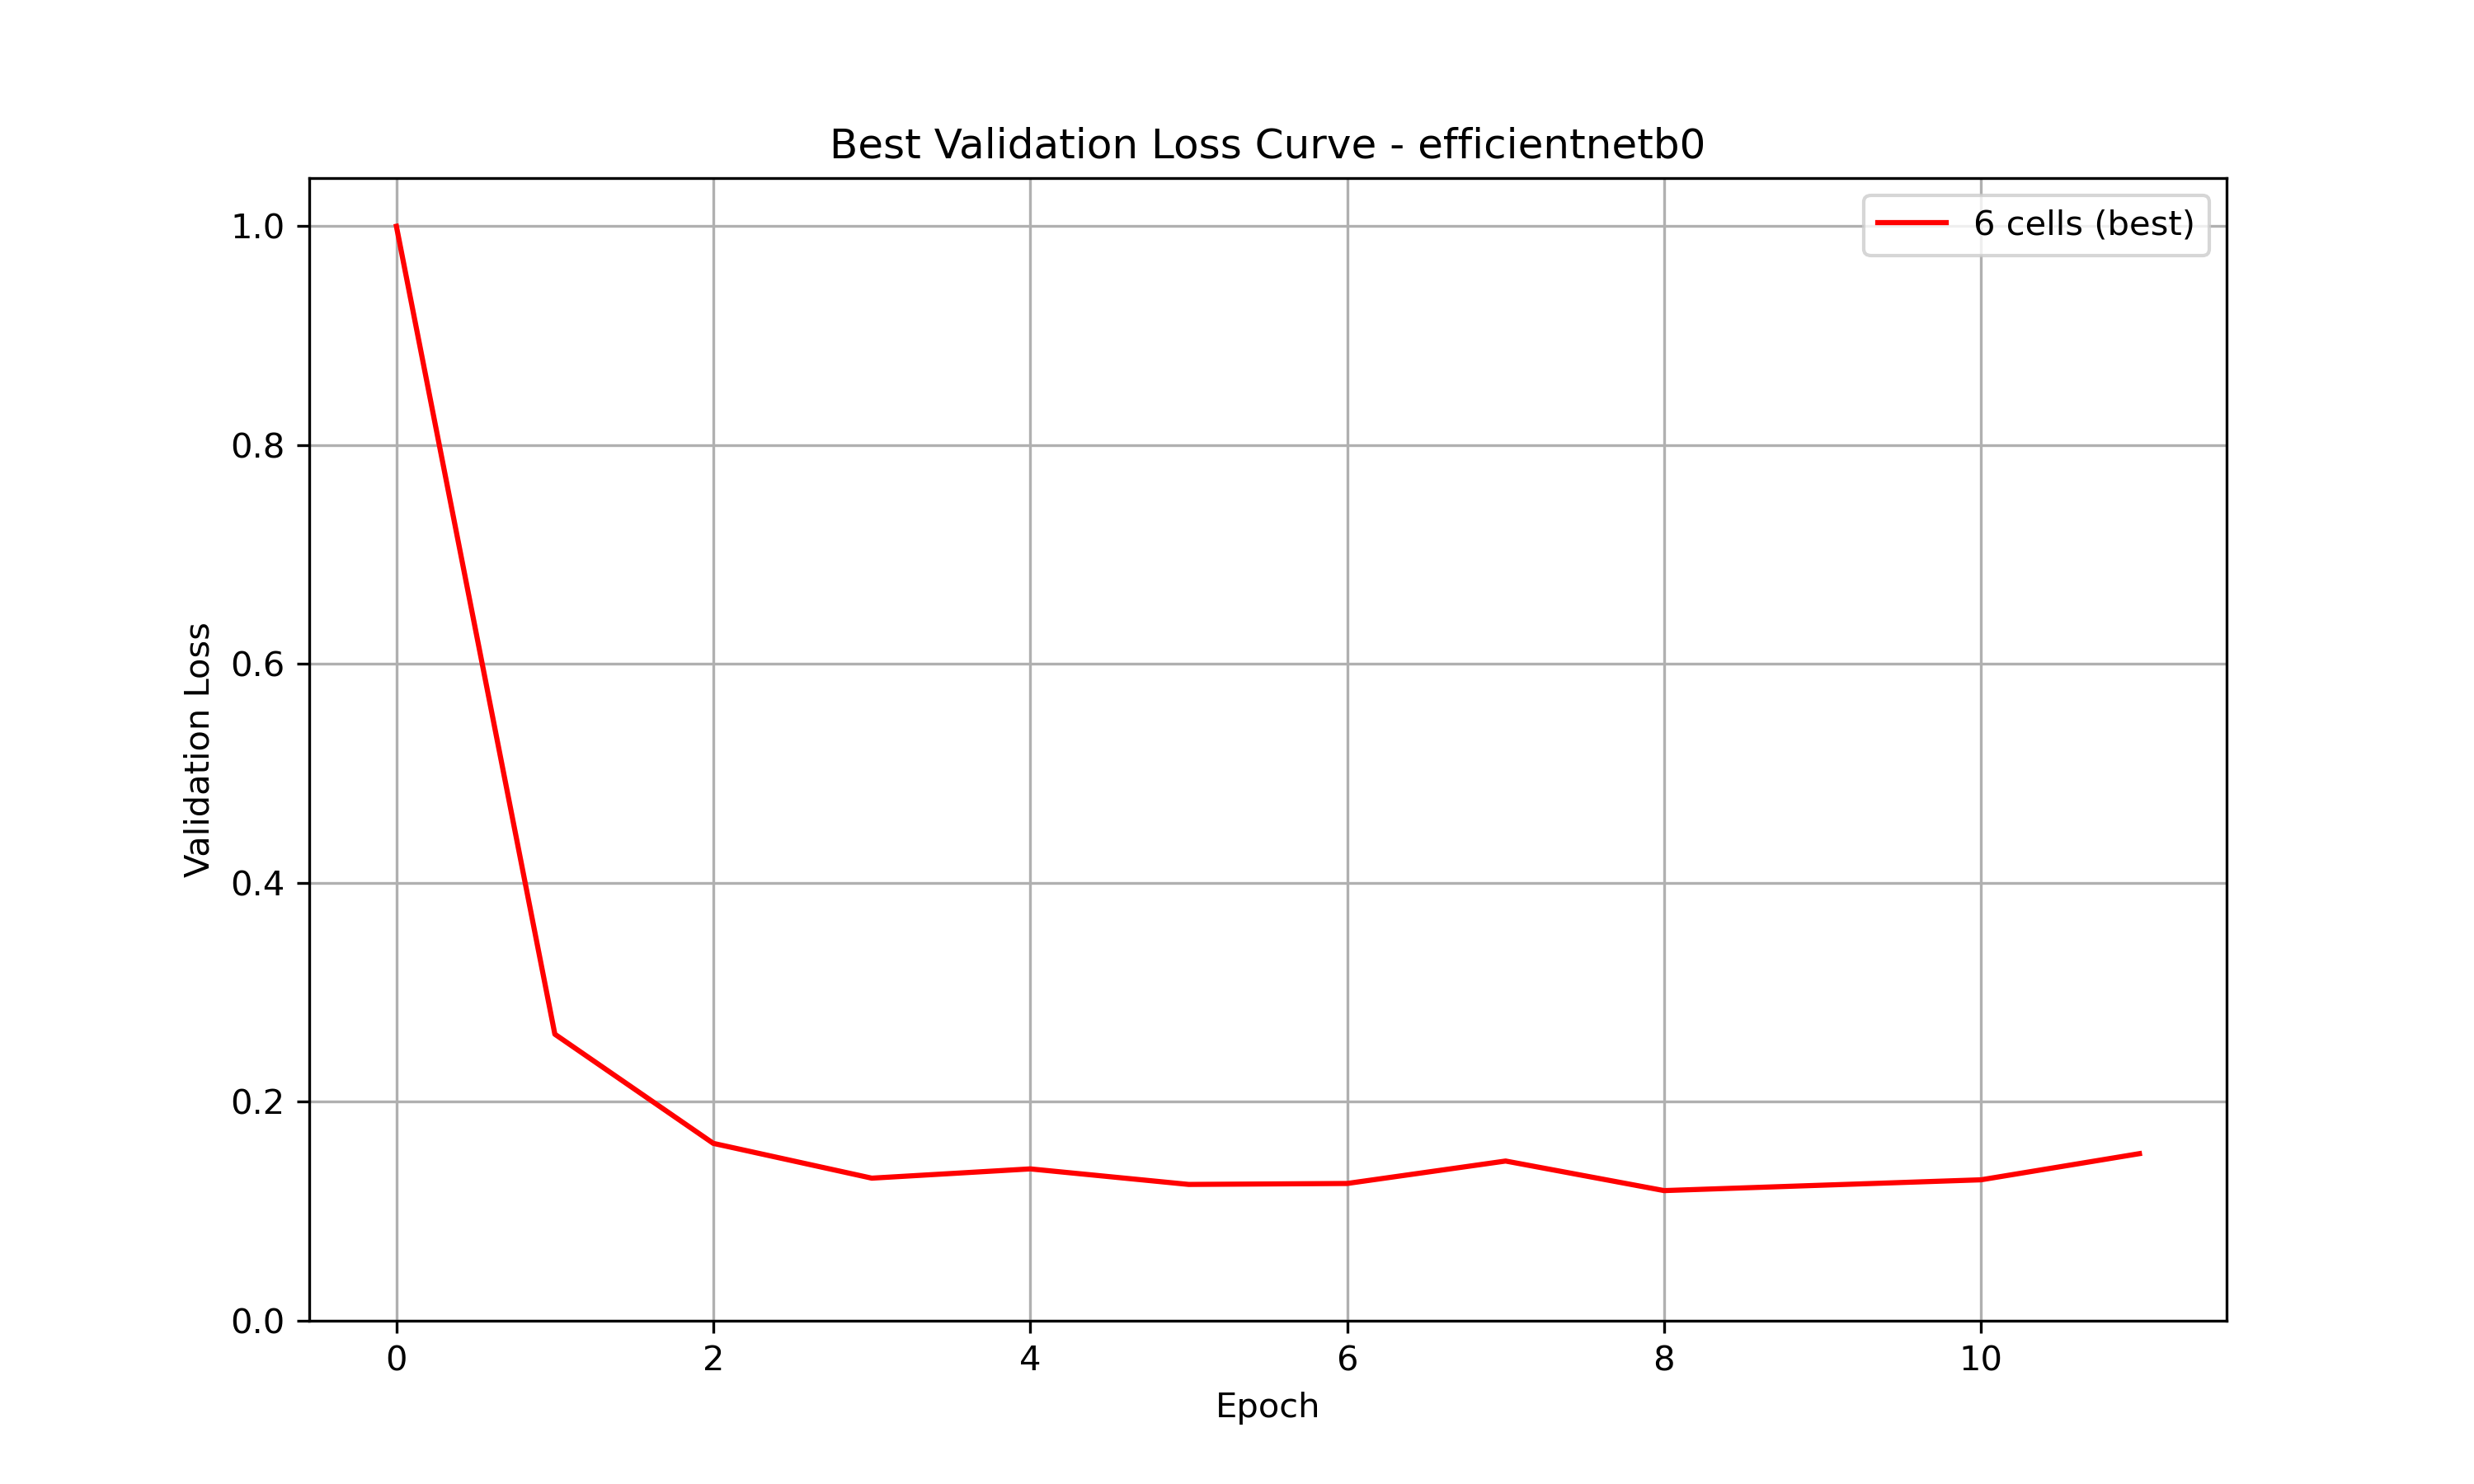
\includegraphics[width=0.8\textwidth]{../graphs/efficientnetb0_best_val_loss.png}
    \centering 
    \caption{Pérdida por época de EfficientNetB0 y 6 capas Bi-LSTM } 
    \label{EfficientNetB0Loss} 
\end{figure}


Los gráficos de las Figuras \ref{EfficientNetB0Accuracy} y 
\ref{EfficientNetB0Loss} muestran lo anteriormente mencionado acerca de 
que el dataset es bastante sencillo como para entrenar un modelo 
para clasificarlo. Durante la primera época, la pérdida baja a alrededor 
de 0.25 mientras que el accuracy logra llegar a 95\% en validación, 
lo cual indica que no está sobreajustandose a los datos de entrenamiento.\\ 

\textbf{\underline{Resultados obtenidos con EfficinetnetV2}}\\

De la misma manera, la Tabla  \ref{table:efficientnetV2Metrics} 
muestra una comparativa entre los resultados obtenidos para el 
\textit{pipeline} manteniendo los vectores de características 
obtenidas a través de EfficientNetV2 de los frames del 
\textit{dataset Hockey Fights}.

\begin{table}[h!]
\centering
\footnotesize
\caption{Métricas obtenidas por configuración de celdas para EfficientNetV2.}
\begin{tabular}{|l|l|l|l|l|l|l|}
\hline
\textbf{\begin{tabular}[c]{@{}l@{}}Celdas \\ Bi-LSTM\end{tabular}} & \textbf{\begin{tabular}[c]{@{}l@{}}Perdida \\ entrenamiento\end{tabular}} & \textbf{\begin{tabular}[c]{@{}l@{}}Accuracy \\ entrenamiento\end{tabular}} & \textbf{\begin{tabular}[c]{@{}l@{}}Perdida \\ validacion\end{tabular}} & \textbf{\begin{tabular}[c]{@{}l@{}}Accuracy \\ validacion\end{tabular}} & \textbf{\begin{tabular}[c]{@{}l@{}}Perdida \\ prueba\end{tabular}} & \textbf{\begin{tabular}[c]{@{}l@{}}Accuracy \\ prueba\end{tabular}} \\ \hline
\textbf{1}                                                         & 0.07                                                                      & 0.99                                                                       & 0.23                                                                   & 0.94                                                                    & 0.11                                                               & 0.97                                                                \\ \hline
\textbf{2}                                                         & 0.08                                                                      & 0.98                                                                       & 0.22                                                                   & 0.94                                                                    & 0.15                                                               & 0.96                                                                \\ \hline
\textbf{3}                                                         & 0.07                                                                      & 0.98                                                                       & 0.26                                                                   & 0.94                                                                    & 0.1                                                                & 0.96                                                                \\ \hline
\textbf{4}                                                         & 0.05                                                                      & 0.99                                                                       & 0.42                                                                   & 0.89                                                                    & 0.09                                                               & 0.98                                                                \\ \hline
\textbf{5}                                                         & \textbf{0.02}                                                             & \textbf{1.0}                                                               & 0.23                                                                   & 0.94                                                                    & \textbf{0.06}                                                      & \textbf{0.99}                                                       \\ \hline
\textbf{6}                                                         & 0.08                                                                      & 0.97                                                                       & 0.34                                                                   & 0.94                                                                    & 0.08                                                               & 0.98                                                                \\ \hline
\textbf{7}                                                         & 0.03                                                                      & 0.99                                                                       & 0.18                                                                   & 0.96                                                                    & 0.08                                                               & 0.98                                                                \\ \hline
\textbf{8}                                                         & 0.1                                                                       & 0.96                                                                       & 0.18                                                                   & 0.94                                                                    & 0.14                                                               & 0.95                                                                \\ \hline
\textbf{9}                                                         & 0.04                                                                      & 0.99                                                                       & \textbf{0.16}                                                          & \textbf{0.96}                                                           & 0.09                                                               & 0.97                                                                \\ \hline
\end{tabular}
\label{table:efficientnetV2Metrics}
\end{table}

En la Tabla \ref{table:efficientnetV2Metrics} se puede observar 
que la configuración que obtuvo el mejor desempeño general fue 
la de 5 celdas Bi-LSTM, alcanzando un \textit{accuracy} del 99\% 
en la prueba. En general, se puede ver que los resultados se mantienen 
consistentes entre configuraciones, con una leve caída en 
rendimiento en el extremo superior con 9 celdas, que mostró el peor 
resultado en prueba (97\% de \textit{accuracy}). Esto sugiere que 
aumentar el número de celdas o introducir un menor número puede 
introducir ruido o sobreajuste.\\

A continuación se presentan las gráficas de pérdida y 
\textit{accuracy} correspondientes a esta configuración óptima.

\begin{figure}[h!] 
    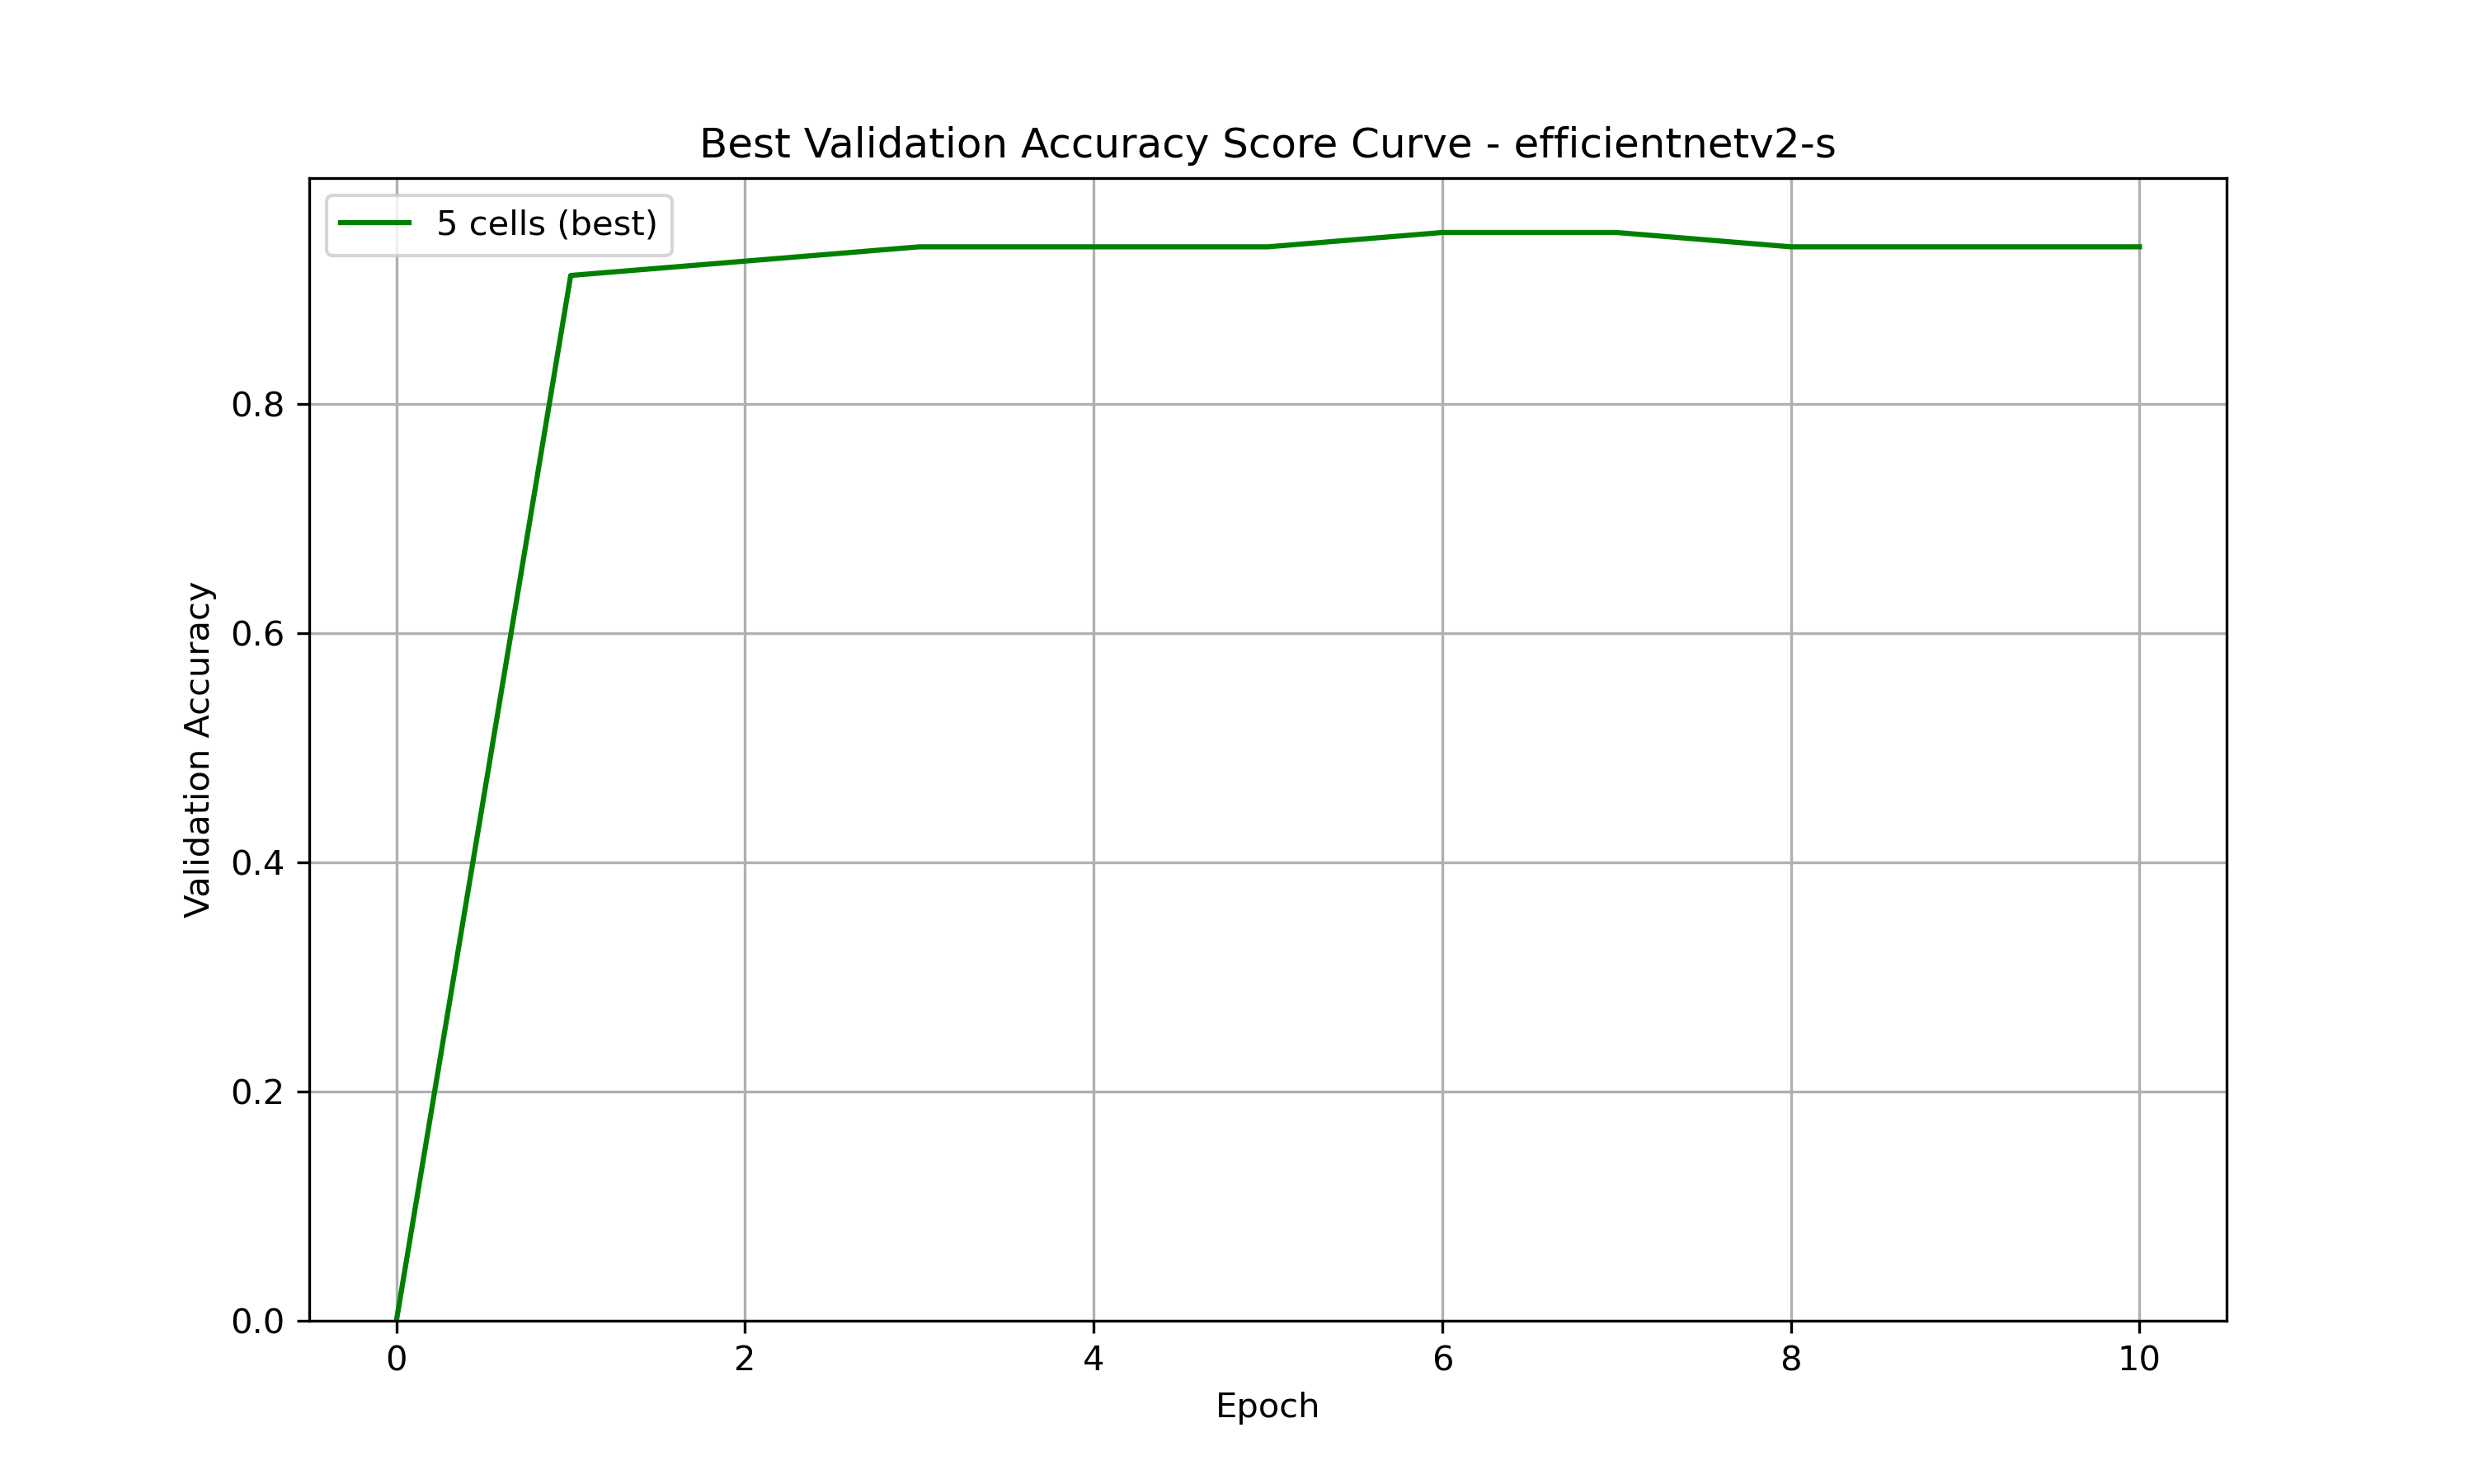
\includegraphics[width=0.8\textwidth]{../graphs/efficientnetv2-s_best_val_accuracy.png} 
    \centering 
    \caption{\textit{Accuracy} por época de EfficientNetV2 y 5 capas Bi-LSTM } 
    \label{EfficientNetV2Accuracy} 
\end{figure}

\begin{figure}[h!] 
    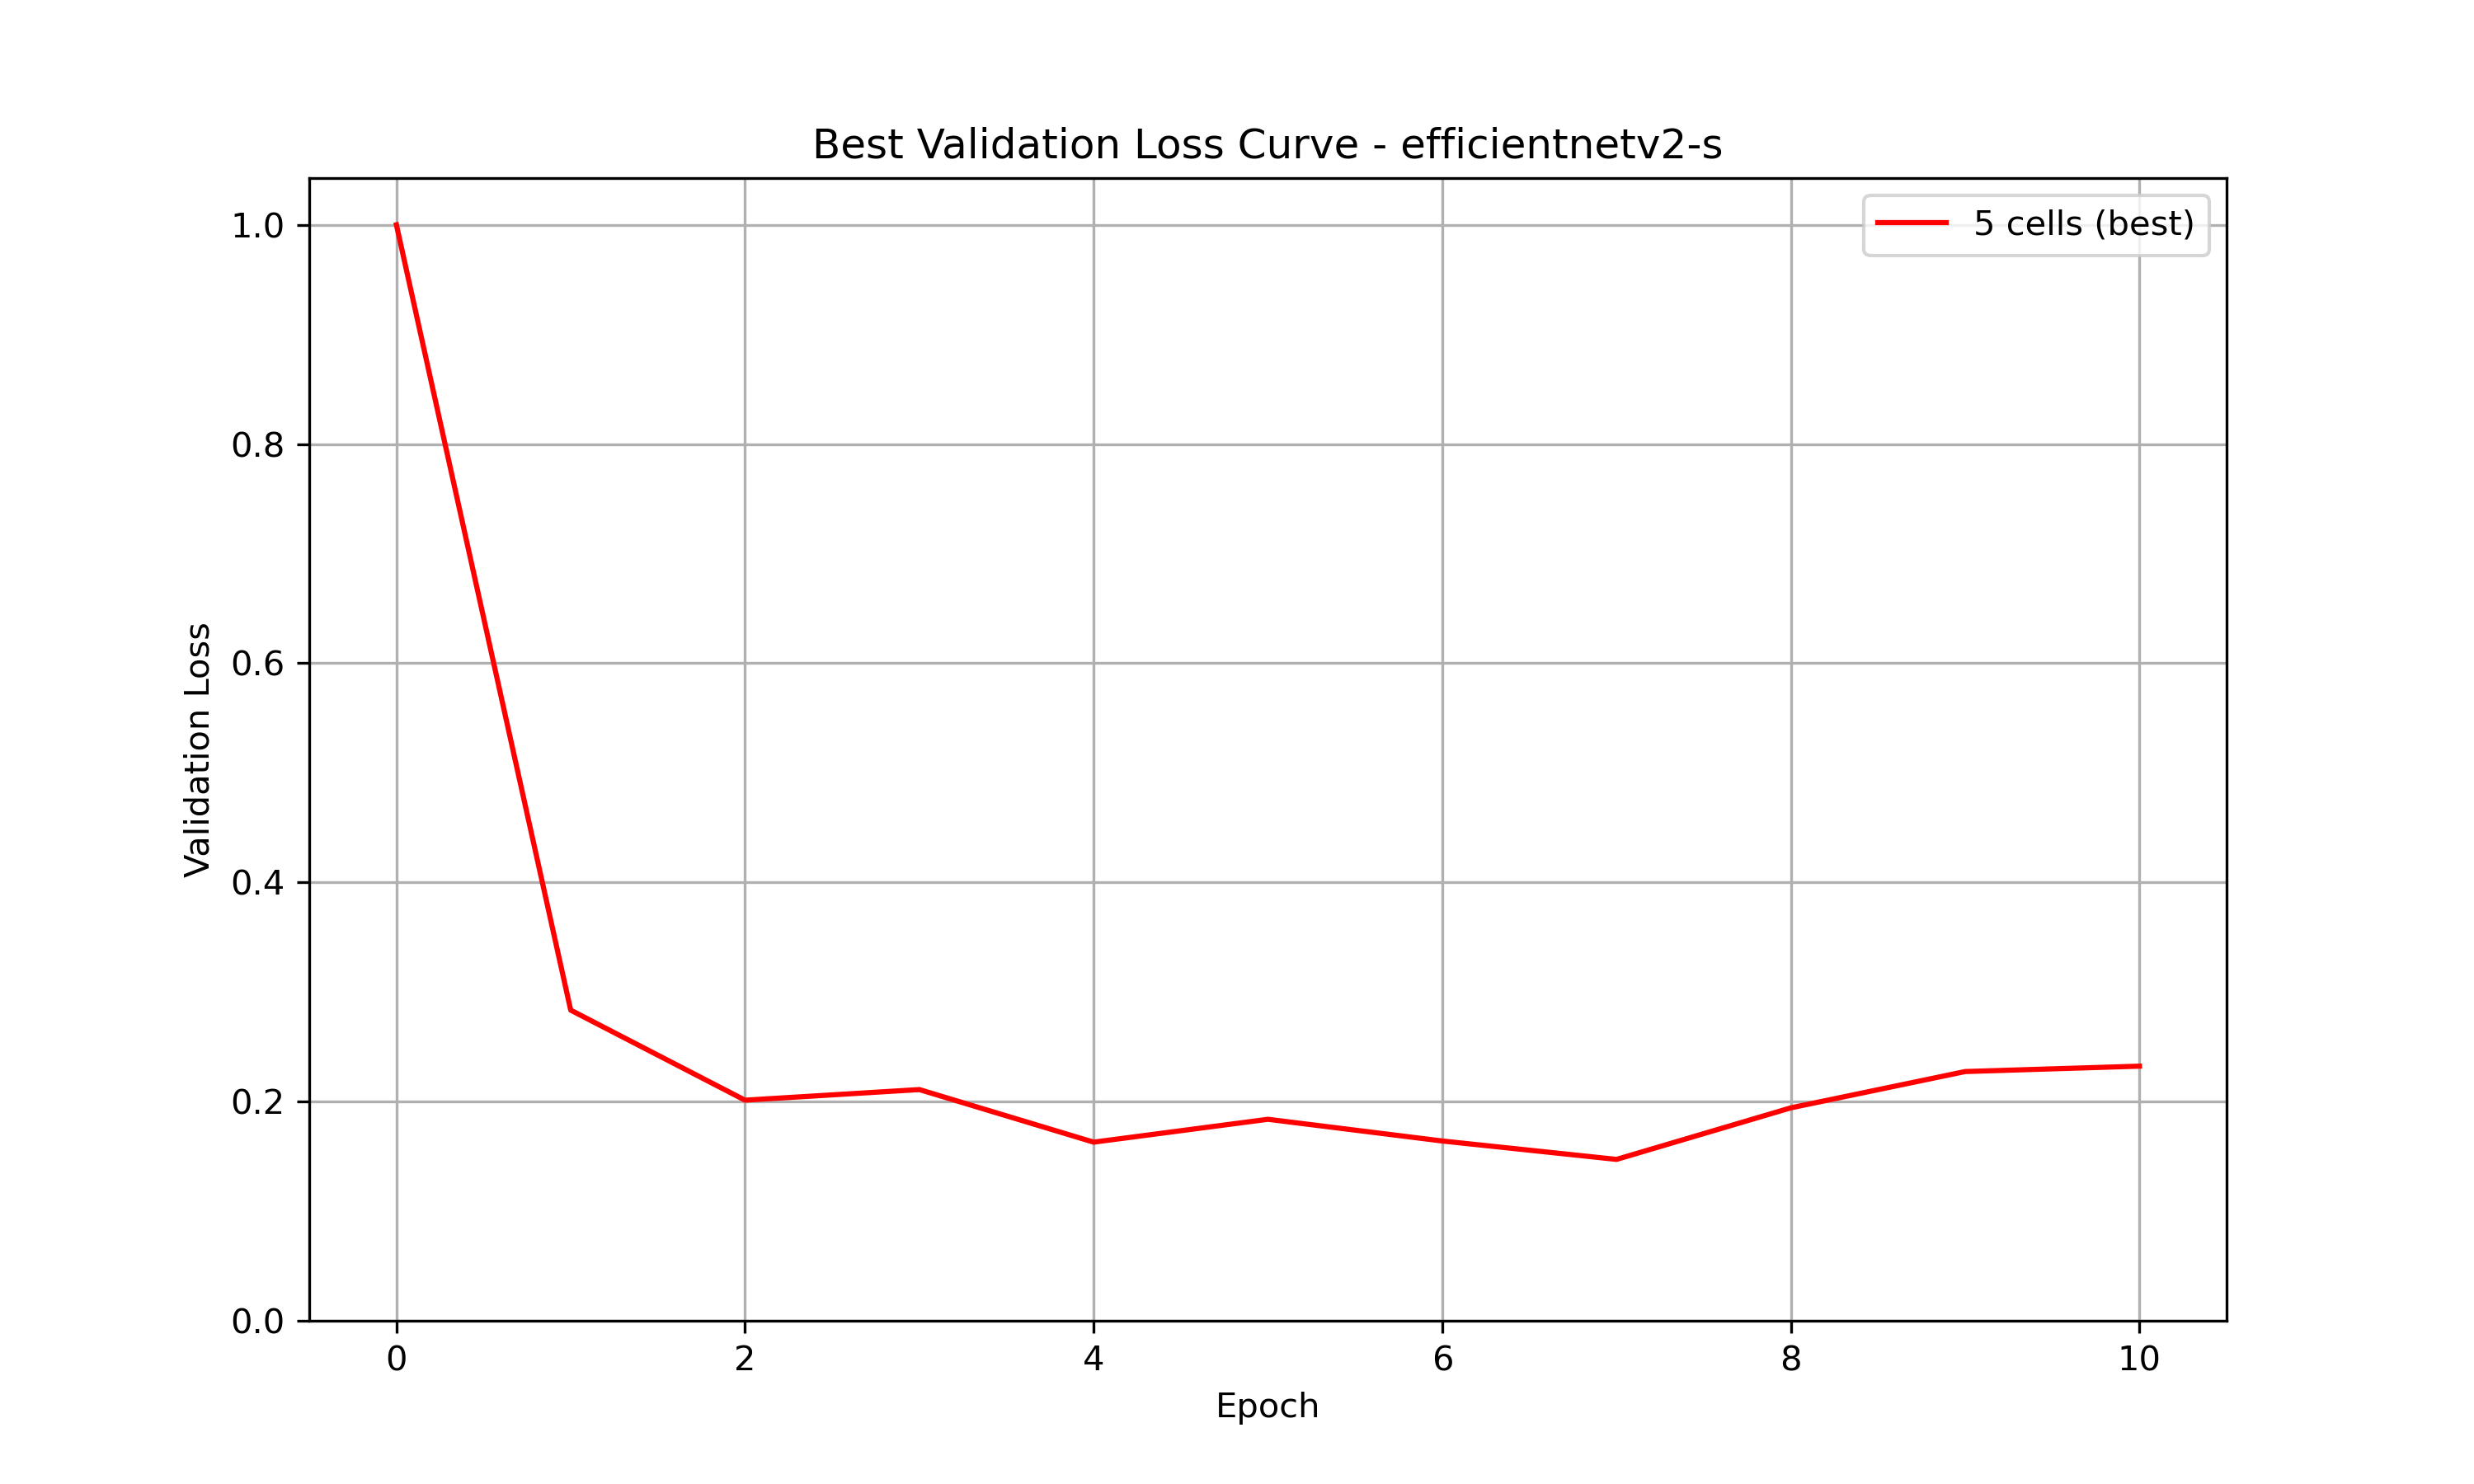
\includegraphics[width=0.8\textwidth]{../graphs/efficientnetv2-s_best_val_loss.png}
    \centering 
    \caption{Pérdida por época de EfficientNetV2 y 5 capas Bi-LSTM } 
    \label{EfficientNetV2Loss} 
\end{figure}


De la misma manera, Los gráficos de las Figuras \ref{EfficientNetV2Accuracy} y 
\ref{EfficientNetV2Loss} muestran el mismo patrón mencionado con los 
experimentos realizados con EfficientNetB0, en donde se obtiene un 
descenso de pérdida y aumento de \textit{accuracy} bastante rápido desde 
la primera época. Durante esta, la pérdida baja a alrededor 
de 0.35 mientras que el accuracy logra llegar a 90\% en validación, 
lo cual indica que no está sobreajustandose a los datos de entrenamiento.\\ 

\textbf{\underline{Resultados obtenidos con MobileNetV3}}\\

A continuación se muestra la Tabla \ref{table:MobileNetV3Metrics} 
la cual conteniendo los resultados obtenidos para el 
\textit{pipeline} manteniendo los vectores de características 
obtenidas a través de \textit{MobileNetV3} de los frames del 
\textit{dataset Hockey Fights}.

\begin{table}[h!]
\centering
\footnotesize
\caption{Métricas obtenidas por configuración de celdas para MobileNetV3.}
\begin{tabular}{|l|l|l|l|l|l|l|}
\hline
\textbf{\begin{tabular}[c]{@{}l@{}}Celdas \\ Bi-LSTM\end{tabular}} & \textbf{\begin{tabular}[c]{@{}l@{}}Perdida \\ entrenamiento\end{tabular}} & \textbf{\begin{tabular}[c]{@{}l@{}}Accuracy \\ entrenamiento\end{tabular}} & \textbf{\begin{tabular}[c]{@{}l@{}}Perdida \\ validacion\end{tabular}} & \textbf{\begin{tabular}[c]{@{}l@{}}Accuracy \\ validacion\end{tabular}} & \textbf{\begin{tabular}[c]{@{}l@{}}Perdida \\ prueba\end{tabular}} & \textbf{\begin{tabular}[c]{@{}l@{}}Accuracy \\ prueba\end{tabular}} \\ \hline
\textbf{1}                                                         & 0.18                                                                      & 0.94                                                                       & 0.24                                                                   & 0.93                                                                    & 0.18                                                               & 0.95                                                                \\ \hline
\textbf{2}                                                         & 0.04                                                                      & \textbf{0.99}                                                              & 0.2                                                                    & 0.94                                                                    & 0.08                                                               & 0.98                                                                \\ \hline
\textbf{3}                                                         & \textbf{0.02}                                                             & \textbf{0.99}                                                              & 0.24                                                                   & 0.95                                                                    & 0.07                                                               & 0.98                                                                \\ \hline
\textbf{4}                                                         & 0.06                                                                      & 0.98                                                                       & \textbf{0.15}                                                          & \textbf{0.96}                                                           & 0.1                                                                & 0.98                                                                \\ \hline
\textbf{5}                                                         & 0.05                                                                      & \textbf{0.99}                                                              & 0.18                                                                   & 0.95                                                                    & 0.1                                                                & 0.97                                                                \\ \hline
\textbf{6}                                                         & 0.07                                                                      & 0.98                                                                       & 0.18                                                                   & 0.94                                                                    & 0.11                                                               & 0.96                                                                \\ \hline
\textbf{7}                                                         & 0.03                                                                      & \textbf{0.99}                                                              & 0.19                                                                   & 0.94                                                                    & 0.08                                                               & 0.97                                                                \\ \hline
\textbf{8}                                                         & 0.06                                                                      & 0.98                                                                       & 0.23                                                                   & 0.94                                                                    & 0.17                                                               & 0.94                                                                \\ \hline
\textbf{9}                                                         & 0.06                                                                      & 0.98                                                                       & 0.19                                                                   & 0.95                                                                    & \textbf{0.05}                                                      & \textbf{0.99}                                                       \\ \hline
\end{tabular}
\label{table:MobileNetV3Metrics}
\end{table}

A comparación de los anteriores dos experimentos, no se logró ver 
ningún patrón característico con respecto al número de capas y la pérdida 
o el \textit{accuracy}. De la misma manera, no se obtuvo un modelo 
sobresaliente en cada una de las etapas de entrenamiento, validación y 
prueba. En ese sentido, se consideró como el mejor modelo al de 9 celdas 
Bi-LSTM debido a su \textit{accuracy} final en prueba, y a continuación 
se muestran las gráficas de pérdida y 
\textit{accuracy} correspondientes.\\

\begin{figure}[h!] 
    \includegraphics[width=0.8\textwidth]{../graphs/MobileNetV3large_best_val_accuracy.png} 
    \centering 
    \caption{\textit{Accuracy} por época de MobileNetV3 y 5 capas Bi-LSTM } 
    \label{MobileNetV3Accuracy} 
\end{figure}

\begin{figure}[h!] 
    \includegraphics[width=0.8\textwidth]{../graphs/MobileNetV3large_best_val_loss.png}
    \centering 
    \caption{Pérdida por época de MobileNetV3 y 5 capas Bi-LSTM } 
    \label{MobileNetV3Loss} 
\end{figure}

A comparación de las otras gráficas se logra ver un entrenamiento menos 
parejos, sobretodo si se ve la Figura \ref{MobileNetV3Loss} en donde 
llegado a la época 4, la gráfica se vuelve anómala en el entrenamiento. \\

\textbf{\underline{Resultados obtenidos con Resnet50}}\\

A continuación se muestra la Tabla  \ref{table:ResNet50} 
la cual conteniendo los resultados obtenidos para el 
\textit{pipeline} manteniendo los vectores de características 
obtenidas a través de \textit{Resnet50} de los frames del 
\textit{dataset Hockey Fights}.\\

\begin{table}[h!]
\centering
\footnotesize
\caption{Métricas obtenidas por configuración de celdas para ResNet50.}
\begin{tabular}{|l|l|l|l|l|l|l|}
\hline
\textbf{\begin{tabular}[c]{@{}l@{}}Celdas \\ Bi-LSTM\end{tabular}} & \textbf{\begin{tabular}[c]{@{}l@{}}Perdida \\ entrenamiento\end{tabular}} & \textbf{\begin{tabular}[c]{@{}l@{}}Accuracy \\ entrenamiento\end{tabular}} & \textbf{\begin{tabular}[c]{@{}l@{}}Perdida \\ validacion\end{tabular}} & \textbf{\begin{tabular}[c]{@{}l@{}}Accuracy \\ validacion\end{tabular}} & \textbf{\begin{tabular}[c]{@{}l@{}}Perdida \\ prueba\end{tabular}} & \textbf{\begin{tabular}[c]{@{}l@{}}Accuracy \\ prueba\end{tabular}} \\ \hline
\textbf{1}                                                         & 0.11                                                                      & 0.97                                                                       & \textbf{0.14}                                                          & \textbf{0.98}                                                           & 0.1                                                                & 0.97                                                                \\ \hline
\textbf{2}                                                         & 0.2                                                                       & 0.94                                                                       & 0.17                                                                   & 0.91                                                                    & 0.19                                                               & 0.94                                                                \\ \hline
\textbf{3}                                                         & 0.08                                                                      & 0.97                                                                       & 0.21                                                                   & 0.93                                                                    & 0.12                                                               & 0.96                                                                \\ \hline
\textbf{4}                                                         & 0.15                                                                      & 0.96                                                                       & 0.17                                                                   & 0.95                                                                    & 0.14                                                               & 0.96                                                                \\ \hline
\textbf{5}                                                         & 0.05                                                                      & 0.98                                                                       & \textbf{0.16}                                                          & \textbf{0.98}                                                           & 0.12                                                               & 0.97                                                                \\ \hline
\textbf{6}                                                         & 0.15                                                                      & 0.96                                                                       & 0.19                                                                   & 0.94                                                                    & 0.2                                                                & 0.95                                                                \\ \hline
\textbf{7}                                                         & \textbf{0.03}                                                             & \textbf{0.99}                                                              & \textbf{0.16}                                                          & 0.96                                                                    & \textbf{0.09}                                                      & \textbf{0.98}                                                       \\ \hline
\textbf{8}                                                         & 0.08                                                                      & 0.98                                                                       & 0.23                                                                   & 0.93                                                                    & 0.16                                                               & 0.94                                                                \\ \hline
\textbf{9}                                                         & 0.08                                                                      & 0.98                                                                       & \textbf{0.16}                                                          & 0.95                                                                    & 0.13                                                               & 0.96                                                                \\   \hline
\end{tabular}
\label{table:ResNet50}
\end{table}


En la Tabla \ref{table:ResNet50} se puede observar 
que la configuración que obtuvo el mejor desempeño casi general fue 
la de 7 celdas Bi-LSTM, alcanzando un \textit{accuracy} del 98\% 
en la prueba. En general, se puede ver que el rendimiento de los modelos 
decae conforme el número de celdas se aleja de 7 en todas las métricas, 
Esto sugiere también que aumentar el número de celdas o introducir 
un menor número puede introducir ruido o sobreajuste.

\begin{figure}[h!] 
    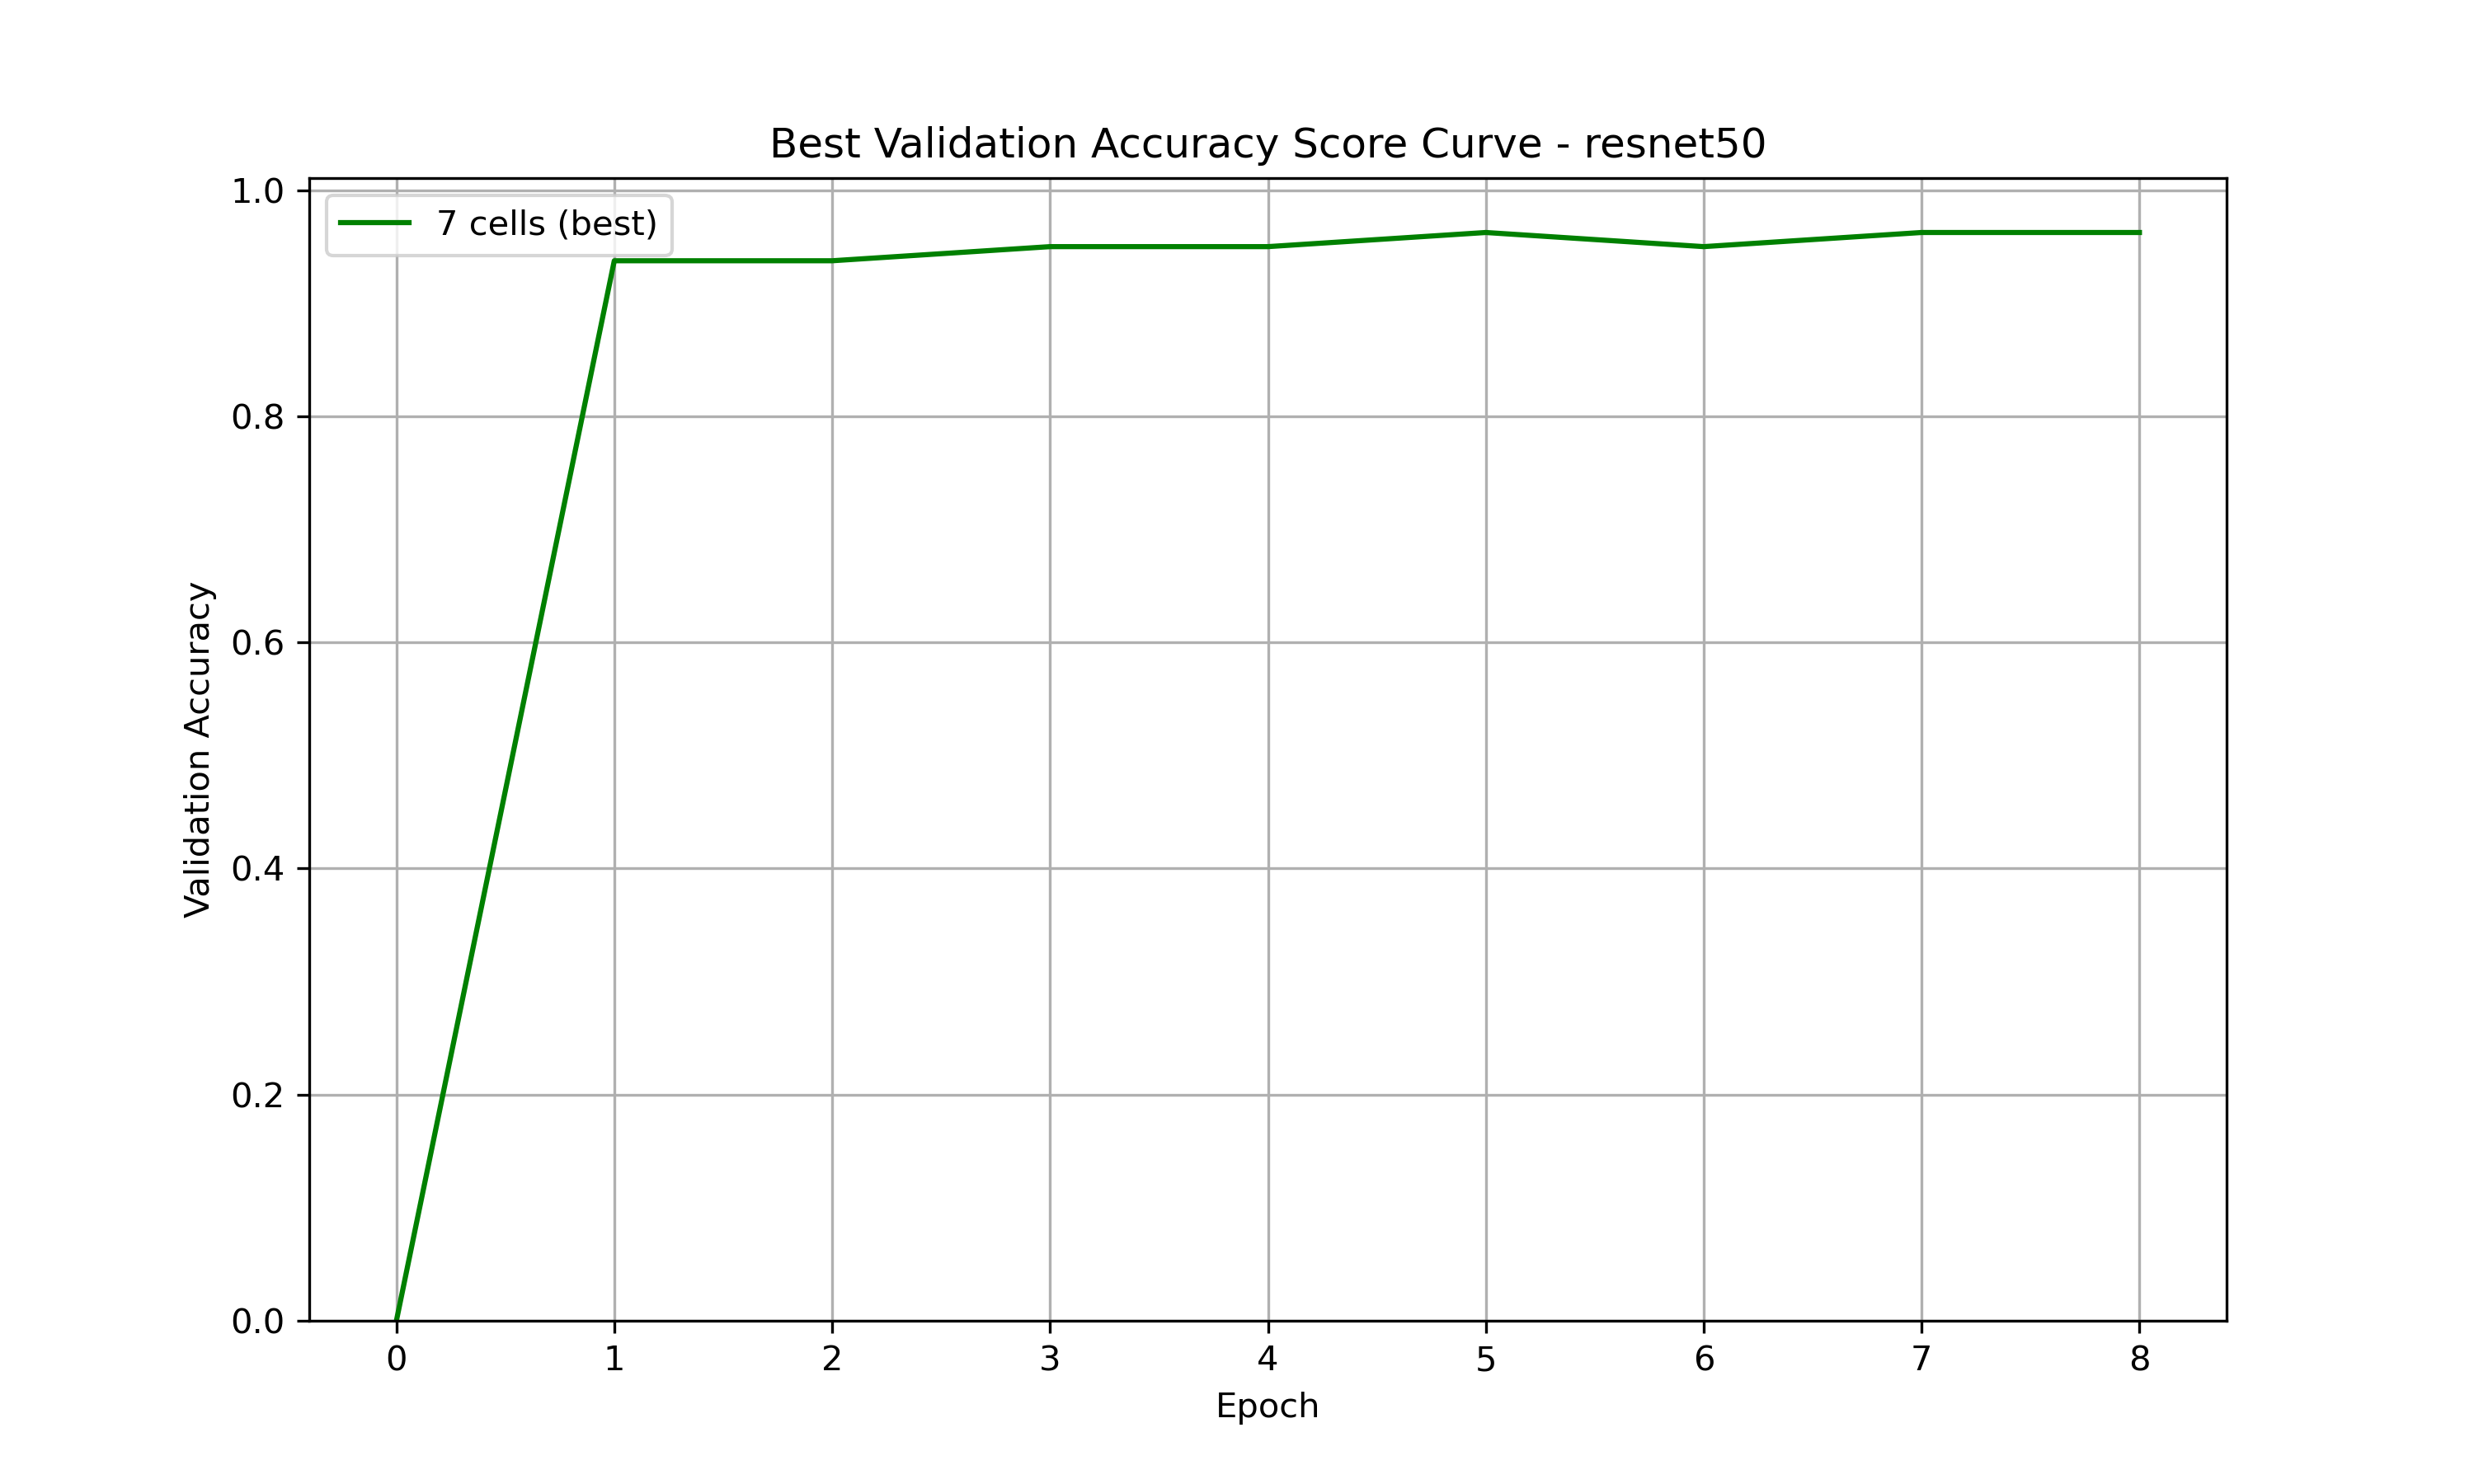
\includegraphics[width=0.8\textwidth]{../graphs/resnet50_best_val_accuracy.png} 
    \centering 
    \caption{\textit{Accuracy} por época de ResNet50 y 7 capas Bi-LSTM } 
    \label{ResNet50Accuracy} 
\end{figure}

\begin{figure}[h!] 
    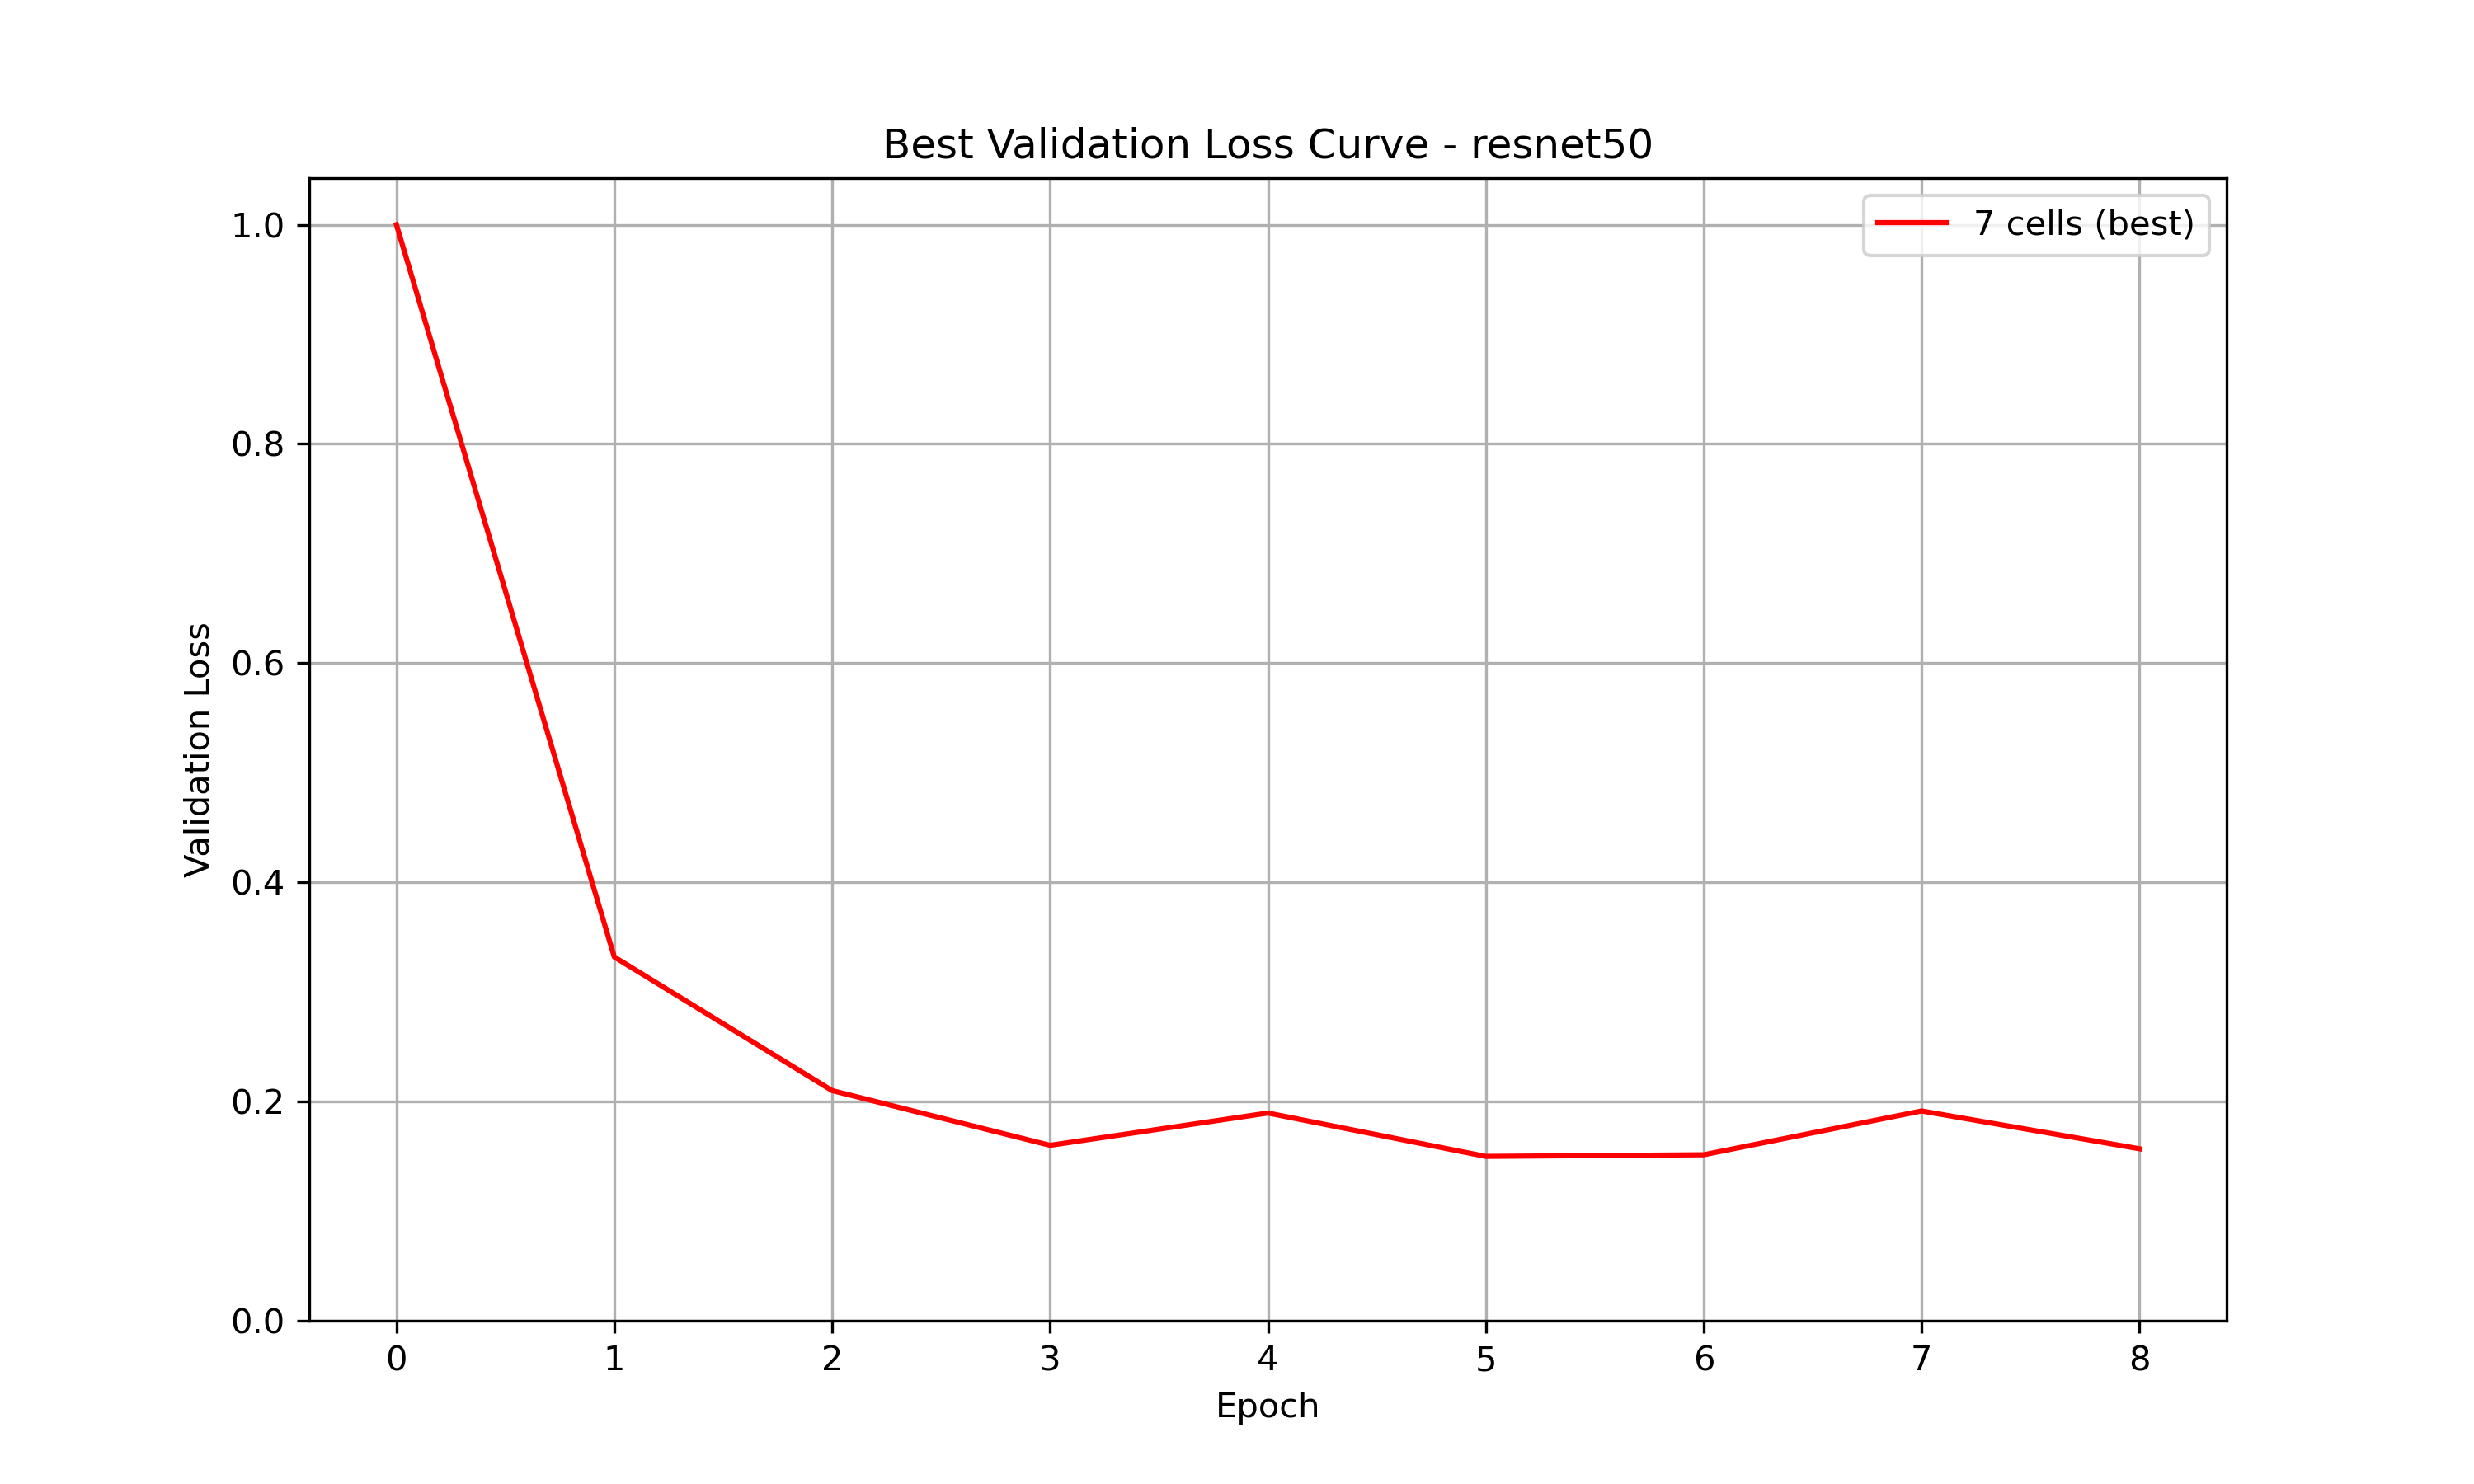
\includegraphics[width=0.8\textwidth]{../graphs/resnet50_best_val_loss.png}
    \centering 
    \caption{Pérdida por época de ResNet50 y 7 capas Bi-LSTM } 
    \label{ResNet50Loss} 
\end{figure}

Al igual que en la anterior experimentación, en la gráfica se logra ver 
un entrenamiento menos parejo, sobretodo si se ve la Figura 
\ref{ResNet50Loss} en donde llegado a la época 4, generando el mismo 
comportamiento anterior.\\

\subsection{Comparativa final}

A continuación se realizará una comparativa a modo de resumen  
de toda la experimentación realizada en el presente trabajo con 
los mejores resultados obtenidos. La Tabla \ref{table:comparacion} 
muestra todas las métricas utilizadas anteriormente para los mejores 
resultados de cada experimento.

\begin{table}[h!]
\centering
\caption{Tabla comparativa resumen final de la experimentación}
{\fontsize{6}{7}\selectfont
\begin{tabular}{|l|l|l|l|l|l|l|l|}
\hline
\multicolumn{1}{|c|}{\textbf{Modelo}} & \textbf{\begin{tabular}[c]{@{}l@{}}Pérdida \\ entrenamiento\end{tabular}} & \textbf{\begin{tabular}[c]{@{}l@{}}Capas \\ Bi-LSTM\end{tabular}} & \textbf{\begin{tabular}[c]{@{}l@{}}Accuracy \\ entrenamiento\end{tabular}} & \textbf{\begin{tabular}[c]{@{}l@{}}Pérdida \\ validación\end{tabular}} & \textbf{\begin{tabular}[c]{@{}l@{}}Accuracy \\ validación\end{tabular}} & \textbf{\begin{tabular}[c]{@{}l@{}}Pérdida \\ prueba\end{tabular}} & \textbf{\begin{tabular}[c]{@{}l@{}}Accuracy \\ prueba\end{tabular}} \\ \hline
\textbf{EfficientNetB0} & 6                    & \textbf{0.00}      & \textbf{1.00}             & \textbf{0.15}   & \textbf{0.98}     & \textbf{0.03}    & \textbf{0.99}     \\ \hline
\textbf{EfficientNetV2} & \textbf{5}           & 0.02               & \textbf{1.00}             & 0.23            & 0.94              & 0.06             & \textbf{0.99}   \\ \hline
\textbf{MobileNetV3}    & 9                    & 0.06               & 0.98                      & 0.19            & 0.95              & 0.05             & \textbf{0.99}   \\ \hline
\textbf{ResNet50}       & 7                    & 0.03               & 0.99                      & 0.16            & 0.96              & 0.09             & 0.98     \\ \hline
\end{tabular}
}
\label{table:comparacion}
\end{table}

Con los resultados finales se puede corroborar que todas las 
combinaciones entre CNN y Bi-LSTM lograron valores similares para 
todas las métricas de testeo al tener un \textit{accuracy} alto y similar 
(98-99\%). Aún así, es importante resaltar que en todas las métricas a lo 
largo del proceso de entrenamiento, validación y prueba, EfficientNetB0 
fue quien obtuvo los mejores resultados en comparación al resto 
(incluyendo el necesitar la menor cantidad de capas Bi-LSTM). En ese 
sentido, y con el fin de optimizar el \textit{pipeline} final de 
manera general, sería recomendable utilizar EfficientNetB0 como extractor 
de características. \\

Por otra parte, y basado en los resultados de todas 
las tablas comparativas anteriormente ilustradas, es recomendable tratar 
de encontrar la configuración con el número de celdas correcto, para 
optimizar el \textit{pipeline} final. Utilizando los patrones 
encontrados, se puede ver que las métricas van a ir mejorando conforme 
más capas se aumente, hasta cierto límite, siendo ese el número ideal 
de capas Bi-LSTM que se debe utilizar.